%Copyright 2014 Jean-Philippe Eisenbarth
%This program is free software: you can 
%redistribute it and/or modify it under the terms of the GNU General Public 
%License as published by the Free Software Foundation, either version 3 of the 
%License, or (at your option) any later version.
%This program is distributed in the hope that it will be useful,but WITHOUT ANY 
%WARRANTY; without even the implied warranty of MERCHANTABILITY or FITNESS FOR A 
%PARTICULAR PURPOSE. See the GNU General Public License for more details.
%You should have received a copy of the GNU General Public License along with 
%this program.  If not, see <http://www.gnu.org/licenses/>.

%Based on the code of Yiannis Lazarides
%http://tex.stackexchange.com/questions/42602/software-requirements-specification-with-latex
%http://tex.stackexchange.com/users/963/yiannis-lazarides
%Also based on the template of Karl E. Wiegers
%http://www.se.rit.edu/~emad/teaching/slides/srs_template_sep14.pdf
%http://karlwiegers.com


\documentclass{scrreprt}

\usepackage{pdfpages}
\usepackage{listings}
\usepackage[T1]{fontenc}
\usepackage{placeins}
\usepackage{float}
\usepackage{underscore}
\usepackage[bookmarks=true]{hyperref}
\usepackage[utf8]{inputenc}
\usepackage{graphicx}
\usepackage{subfigure}
\usepackage[english]{babel}
\hypersetup{
	bookmarks=false,    % show bookmarks bar?
	pdftitle={Software Requirement Specification},    % title
	pdfauthor={Adam-Ryan},                     % author
	pdfsubject={TeX and LaTeX},                        % subject of the document
	pdfkeywords={TeX, LaTeX, graphics, images}, % list of keywords
	colorlinks=true,       % false: boxed links; true: colored links
	linkcolor=blue,       % color of internal links
	citecolor=black,       % color of links to bibliography
	filecolor=black,        % color of file links
	urlcolor=blue,        % color of external links
	linktoc=page            % only page is linked
}%
\def\myversion{1 }
\date{}
%\title
\usepackage{hyperref}
\begin{document}
	
	\begin{flushright}
		\rule{16cm}{5pt}\vskip1cm
		\begin{bfseries}
			\Huge{Tutorial 1\\}
			\vspace{1.9cm}
			for\\
			\vspace{1.9cm}
			Data Mining - Exploration and Pre-processing
			\vspace{1.9cm}
			\LARGE{Version \myversion}\\
			\vspace{1.9cm}
			Adam Ryan (14395076)\\
			\vspace{1.9cm}
			COMP47530\\
			\vspace{1.9cm}
			\today\\
		\end{bfseries}
	\end{flushright}
	
	\tableofcontents

	
\chapter{Question 1}
\section{Exercise 1 - Questions}\label{E1Q}
An analyst collects surveys from different participants about their likes and dislikes.
Subsequently, the analyst corrects erroneous or missing entries, uploads the data to a data warehouse, and designs a recommendation algorithm on this basis.
\\
\\
Which of the following actions represent data collection, data preprocessing, and data analysis?
\begin{itemize}
\item Conducting surveys and uploading to a database.
\item Correcting missing entries.
\item Designing a recommendation algorithm.
\end{itemize}

	
\section{Question 1 - Answer}
This is the answer to question one on the tutorial sheet. In the three example provided within the question above, the following is the mapping

\begin{itemize}
\item Conducting surveys and uploading to a database. - This is data collection, as the analyst is collecting the data which they are going to use in their analysis.
\item Correcting missing entries. - This is data preprocessing, as it is the cleansing of data in order to prepare for the subsequent analysis.
\item Designing a recommendation algorithm. - This is data analysis, as it is the creation of models following the processing of data which includes the analysis and model generation of the data. This process is typically iterative.
\end{itemize}



\newpage
\chapter{Question 2}
\section{Exercise 2 - Questions}\label{E2Q}

One of the important aspects of data collections is that they contain a wide variety of data types, which should be taken into account during the analysis. From the analysis point of view, we can distinguish two broad categories of data: Non-dependency-oriented data, and Dependency-oriented data.
\\
\\
\textbf{Non-dependency-oriented data}: The data records do not have any specific dependencies between either the data items or the attributes. A record is referred to as data point, instance, example, transaction, entity, tuple, object, or feature- vector. Each record contains a set of fields, which are also referred to as attributes, dimensions, and features. Non-dependency-oriented data is the simplest form of data and typically refers to multidimensional data.
We can have attributes of different types of data. These include numeric data, categorical data, binary data, text data.
\\
\\
\textbf{Dependency-oriented data}: the data contains implicit or explicit relationships. In the case of implicit dependencies, the relationship is not expressed in the data. For example consecutive reading of temperature values, that are close in time, are more likely to be similar. Explicit dependencies refer to graph or network data in which edges are used to specify explicit relationships.
\\
\\
Different types of dependency-oriented data are: Times-Series Data, Discrete Sequences and Strings, Spatial Data, Spatio-temporal Data, and Network and Graph Data.
\\
\\
The same analyst obtains medical notes from a physician for data mining purposes, and then transforms them into a table containing the medicines prescribed for each patient. What is the data type of
\begin{enumerate}
\item The original data?
\item The transformed data?
\item What is the process of transforming the data to the new format called?
\end{enumerate}


\section{Exercise 2 - Answers}
This is solution to the question in Exercise 2. 
\begin{enumerate}
	\item The original data - The original data is known as the raw data.
	\item The transformed data - This is the staged data (otherwise known as cleansed/processed/transformed data).
	\item What is the process of transforming the data to the new format called? - This is the data pre-processing stage (otherwise known as data transformation or data cleansing stage).
\end{enumerate}

 \noindent In terms of categorising the type of data in the context of dependency-oriented vs non-dependency-oriented, this is not clearly possible to classify without more detail on the actual data which is being obtained. For example, if the medical notes are time-series data charting the patients' vitals over time with respect to certain medicines, the data is implicitly dependency-oriented, and similarly if the medicines which are prescribed are expected to have interactions or are for a common issue it may be dependency-oriented. If the medical notes are separate treatments over time then it may be considered transactions in a EMS system such as EPIC where the data is as non-dependency-oriented data, however classifying the data into either category based on the terms given as it could theoretically fall into either category, and likewise the cleansed data depends on exactly how it's being listed. My assumption as to how the question is expecting us to answer is below:
\begin{enumerate}
	\item The original data - Dependency-oriented data as each medical note is inherently written in the context of what has come previously (e.g. what medicines and treatments the patient has been previously prescribed and how they have reacted)
	\item The transformed data - Dependency-oriented data as there is an inherent dependency between the medicines which the patient is on, the severity of the illness, and their reaction to prior medicines.
	\item What is the process of transforming the data to the new format called? - This is the data pre-processing stage (otherwise known as data transformation or data cleansing stage).
\end{enumerate}

	
\newpage	
\chapter{Question 3}
\section{Exercise 3 - Questions}
Suppose that the data for analysis includes the attribute age. The age values for the data tuples are (in increasing order):
\\
\\
13, 15, 16, 16, 19, 20, 20, 21, 22, 22, 25, 25, 25, 25, 30, 33, 33, 35, 35, 35, 35, 36, 40, 45, 46, 52, 70
\begin{enumerate}
\item What is the mean of the data? What is the median?
\item What is the mode of the data? Comment on the data’s modality (i.e., bimodal, trimodal, etc.). 
\item What is the midrange of the data?
\item Can you find (roughly) the first quartile (Q1) and the third quartile (Q3) of the data?
\item Give the five-number summary of the data.
\item Show a boxplot of the data.
\item How is a quantile-quantile plot different from a quantile plot?
\end{enumerate}




\section{Exercise 3 - Answers}	
The following are the answers to exercise 3 in the first tutorial sheet:

\begin{enumerate}
	\item The mean of the data is 29.96 (to two decimal places) and the median is 25. The mean is arrived at by summing all values over the total, while the median is arrived at by ordering all data points and choosing the 'middle' value.
	\item The mode of the data is 25 and 35 as both values occur four times which is more than any other value in the data set. The mode is arrived at by counting the occurrence of each value and identifying the values which occur most commonly. The value is bimodal as there are two modes, however we can see the data overall is skewed towards lower age groups.
	\item The range of the data is 57 and the mid-range is 28.5. This is half of the sum of the max and min values within the dataset.
	\item The first quartile of the dataset is 20.5 and the third quartile is 35.
	\item The following is the five-number summary of the dataset. This is arrived by combining the data we have from the previous answers.
	\begin{itemize}
	\item minimum=13 
	\item Q1=20.5 
	\item median=25.0 
	\item Q3=35.0 
	\item maximum=70
	\end{itemize}
	\item The boxplot of the data has been printed below by using pandas' default plotting functionality which leverages matplotlib and is a standard method of accomplishing this.
\begin{figure}[h]
	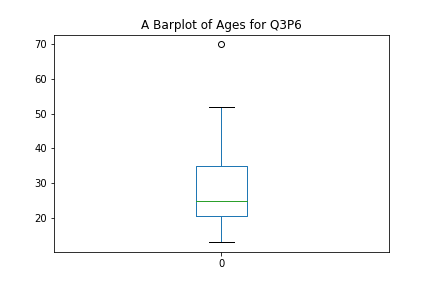
\includegraphics[width=8cm]{Q3P6_Barplot}
	\centering
\end{figure}
	\item A quantile-quantile plot is a plot which is used to determine if multiple datasets follow the same distribution. Depending on the distribution which is being checked for, if both quantities are from the same distribution then the plots should fall along the same path. A quantile plot, on the otherhand, involves looking at your single dataset and using linear interpolation to create quantiles of your dataset and plotting the values against the quantile to visualise the data's distribution.
\end{enumerate}


	
\newpage
\chapter{Question 4}
\section{Exercise 4 - Question}
The file AutoMpg question1.csv contains data related to cars, such as horsepower, weight, car name, and so on. Unfortunately, some of the values for the horsepower and origin columns were not properly recorded. Can you tell how many missing values are there for each one of these columns? Write the answer in your report.

\begin{enumerate}
\item Replace the missing horsepower values with the average of this column.
\item Replace the missing origin values with the minimum of this column
\item Save the generated data file to ./output/question1 out.csv
\end{enumerate}

When saving the generated data, pay extra attention to the columns included in the file (hint: if you are using pandas, take a look at the arguments of the to\_csv function).


\section{Exercise 4 - Answers}
The following details my notes on Exercise 4.
	\begin{enumerate}
		
		\item There were 16 missing horsepower values and 15 missing origin values
		\item Replace the missing horsepower values with the average of this column - I use pandas series mean to compute the mean of the non-null horsepower values. I use the fillna function in order to replace all na values with the mean value. By reading the CSV as a dataframe it is easy to achieve this functionality.
		\item Replace the missing origin values with the minimum of this column- I use pandas series min to compute the minimum of the non-null origin values. I use the fillna function in order to replace all na values with the minimum value. By reading the CSV as a dataframe it is easy to achieve this functionality.
		\item Save the generated data file to ./output/question1 out.csv - I use the to\_csv function to save the resulting dataframe to a CSV file. I ensure the index is not saved as this was not in the original dataset.
	\end{enumerate}
	
	
	
	
\newpage
\chapter{Question 5}
\section{Exercise 5 - Questions}

The files AutoMpg question2 a.csv and AutoMpg question2\_b.csv contain similar pieces of information about car models. There are some differences between the 2 files. What you need to do is:
\begin{enumerate}
\item The dataset A has an attribute called car name, whereas the dataset B has an attribute called name. Rename the name attribute to car name (unintended tongue twister!).
\item The dataset B has an attribute called other, which is not present in the dataset A. Create an attribute called other in the dataset A and assign it a default value of 1.
\item Concatenate dataset A and B together, and just like in question 1, save the resulting file to ./output/question2\_out.csv.
\end{enumerate}


\section{Exercise 5 - Answers}
This section details my answers to question 5.
\begin{enumerate}
	\item The dataset A has an attribute called car name, whereas the dataset B has an attribute called name. Rename the name attribute to car name (unintended tongue twister!). - I use pandas column rename functionality on the dataset to accomplish this.
	\item The dataset B has an attribute called other, which is not present in the dataset A. Create an attribute called other in the dataset A and assign it a default value of 1. - I add in the column using standard pandas notation and set it to 1 as described.
	\item Concatenate dataset A and B together, and just like in question 1, save the resulting file to ./output/question2\_out.csv. - I use the concatenation function to concatenate dataframe b onto dataframe a and then I save it without the index.
\end{enumerate}


	
\end{document}
